\section{XML}

\subsection{Wat is XML?}

XML = eXtensible Markup Language

\subsection{Geef een voorbeeld van XML}

\begin{figure}[h!]
\centering
  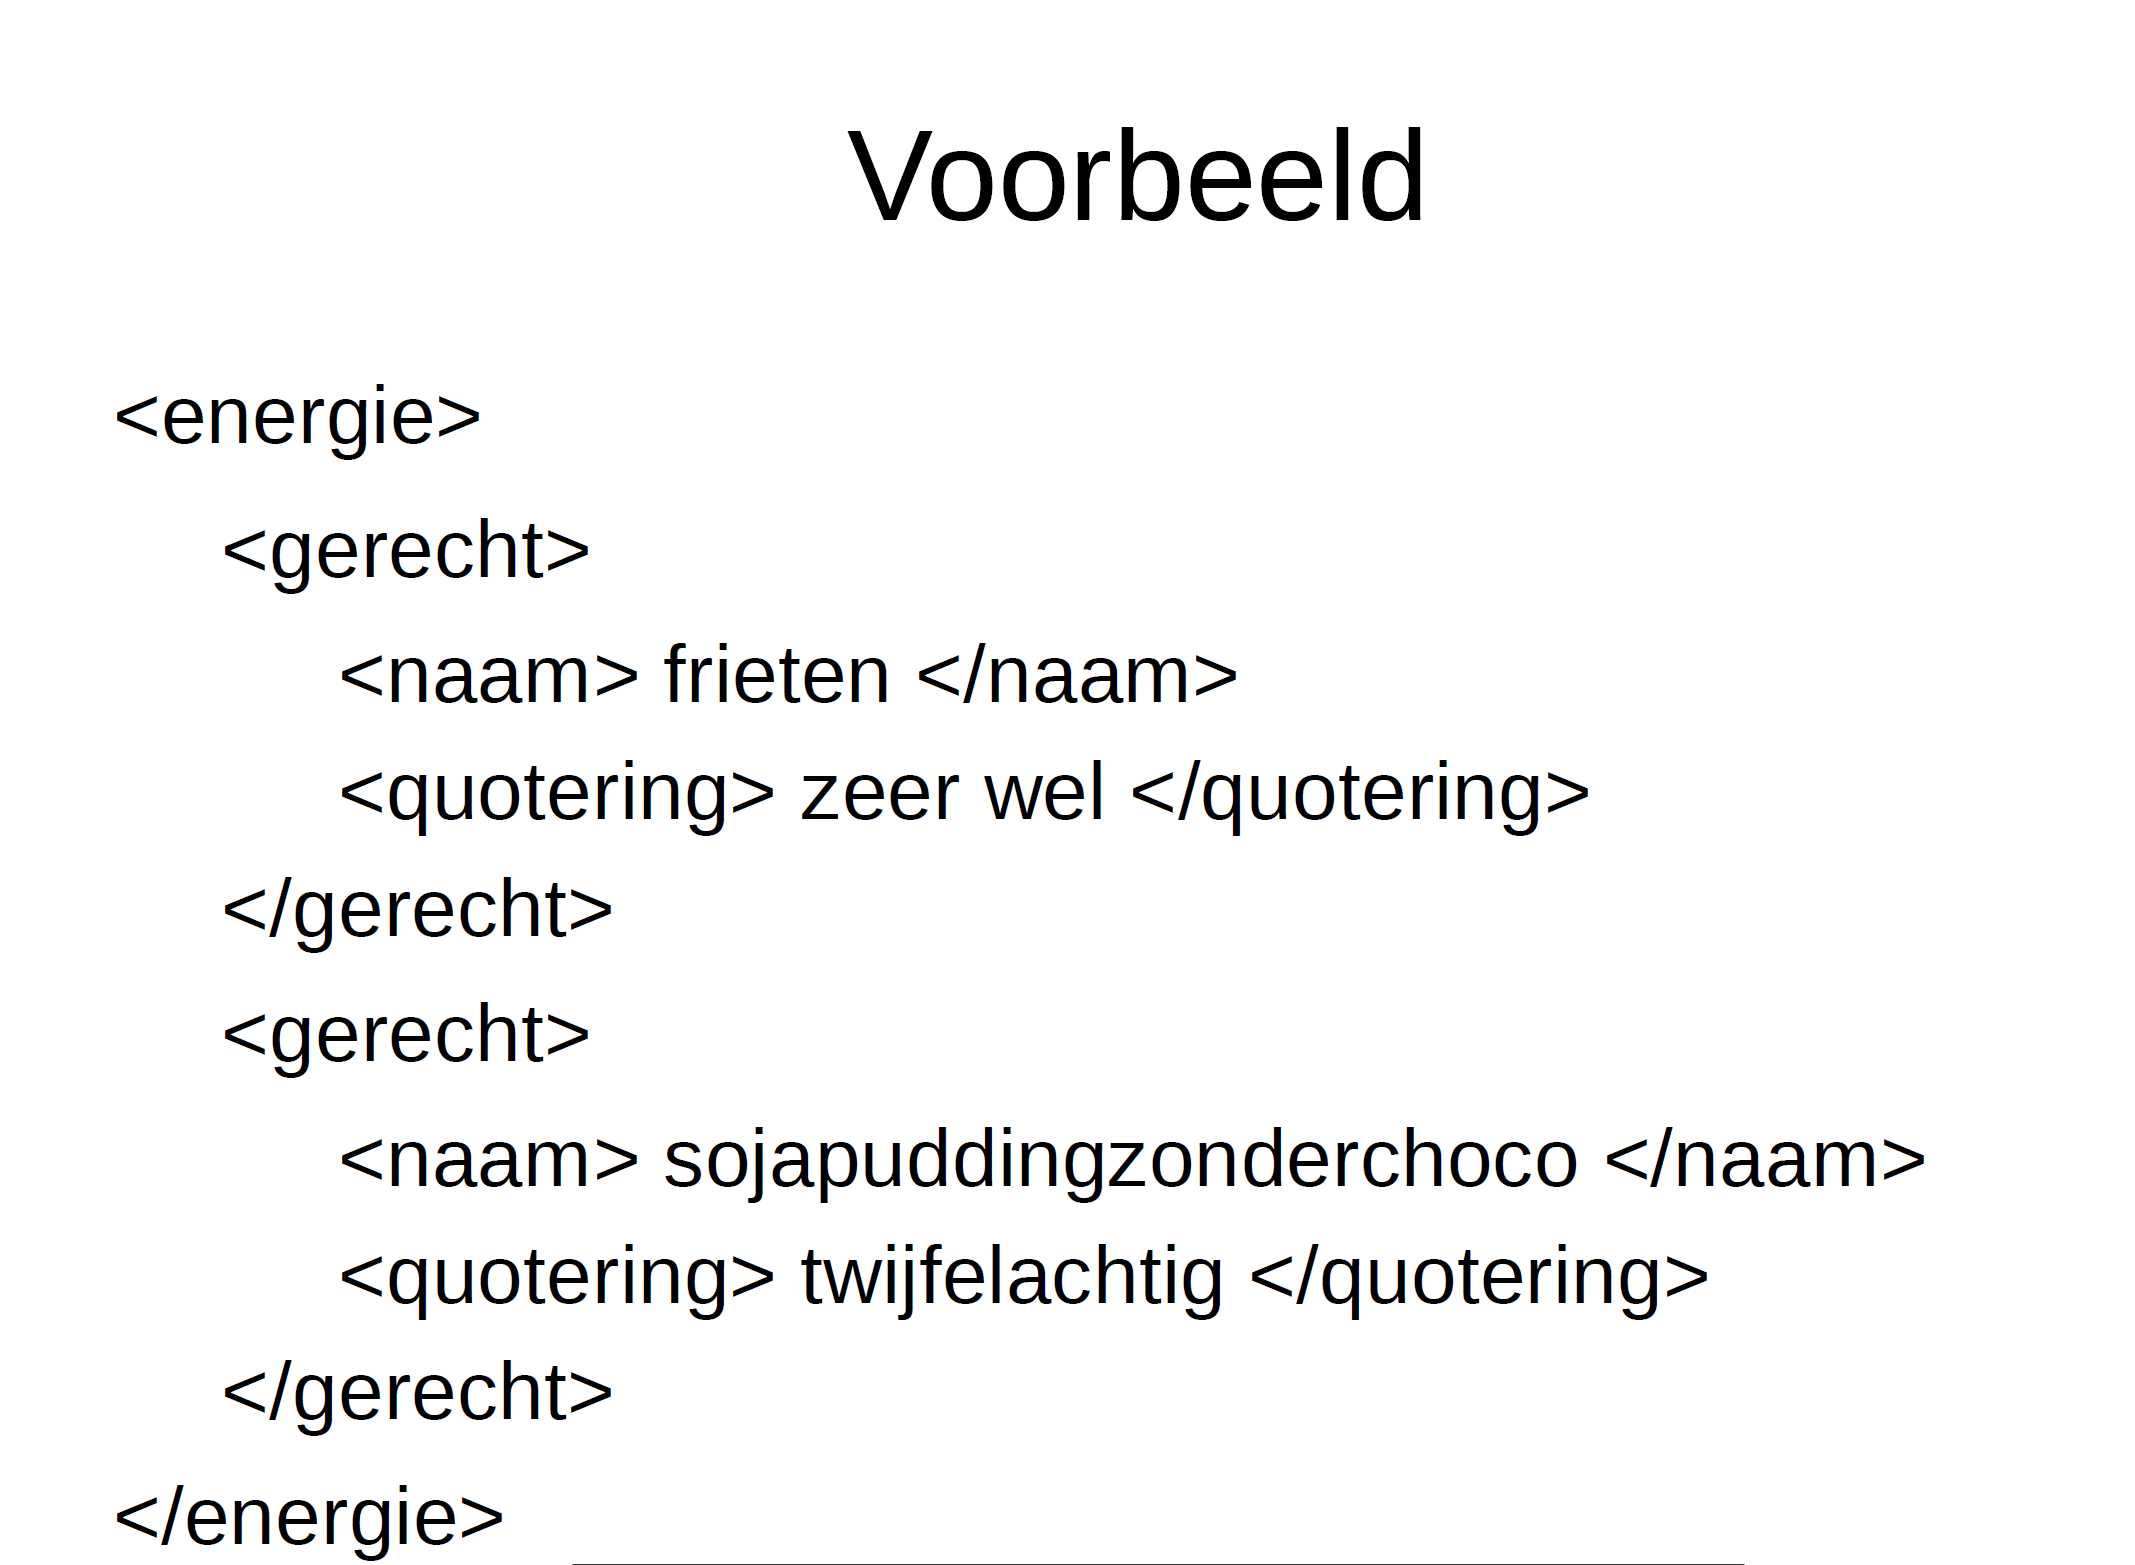
\includegraphics[width=0.5\textwidth]{./figures/xml.png}
  \caption{XML voorbeeld.}
  \label{fig:xml}
\end{figure}

%Figure \ref{fig:boat1} shows a boat.

\subsection{Wat is het doel van (meerdere) XML bestanden?}

\begin{itemize}
    \item om zowel hiërarchische datastructuren te omschrijven als deze te bevatten
    \item om data uit wisselen tussen verschillende gegevensbronnen
\end{itemize}

\subsection{Voordelen van XML voor dataopslag}

\begin{itemize}
\item ISO
\item Uitwisselbaarheid
\item Eenvoud
\item Geen hierarchische engine nodig
\end{itemize}

\subsection{Nadelen van XML voor dataopslag}

\begin{itemize}
\item Redundantie ten opzichte van relationeel model, dus niet misbruiken in die zin
\item Sequentieel
\item Traag
\item ...
\end{itemize}

\subsection{Wat is RSS?}
RSS = Really Simple Syndication.
Alle RSS-varianten zijn XML-bestanden, RSS-feeds genaamd.

Voorbeeld:

\begin{minted}{xml}
<?xml version="1.0"?>
<rss version="2.0">
  <channel>
    <title>Wikipedia Nederland - Nieuwe artikelen</title> 
    <link>//nl.wikipedia.org/</link> 
    <description>Deze webfeed notificeert u van nieuwe 
    artikelen op Wikipedia NL.
    </description>
    <item>                                                                                                                                                 
      <title>RSS</title> 
      <link>//nl.wikipedia.org/wiki/Really_Simple_Syndication</link> 
      <description>RSS, of Really Simple Syndication,
      is een familie van webfeedformaten.</description> 
    </item>
    <item>
      <title>Atom</title> 
      <link>//nl.wikipedia.org/wiki/Atom</link> 
      <description>Atom is een soort webfeed, net als RSS.</description> 
    </item>
  </channel>
</rss>
\end{minted}

\noindent Links:

\noindent \href{https://nl.wikipedia.org/wiki/Really_Simple_Syndication}{RSS wikipedia nederlands}\\
\href{https://en.wikipedia.org/wiki/RSS}{RSS wikipedia engels}

\subsection{SQL functies voor XML}

Zie slides 06 \_\ 3XML.PDF